\documentclass{article}
% ------------ xcolor ----------- %
\usepackage[usenames,dvipsnames,svgnames,table]{xcolor}
\definecolor{lightgrey}{rgb}{0.96,0.97,0.98}
% if you need to pass options to natbib, use, e.g.:
% \PassOptionsToPackage{numbers, compress}{natbib}
% before loading nips_2016
%
% to avoid loading the natbib package, add option nonatbib:
% \usepackage[nonatbib]{nips_2016}
% to compile a camera-ready version, add the [final] option, e.g.:
% \usepackage[final]{nips_2016}
\usepackage[]{nips_2016}
\usepackage[utf8]{inputenc} % allow utf-8 input
\usepackage[T1]{fontenc}    % use 8-bit T1 fonts
\usepackage{hyperref}       % hyperlinks
\usepackage{url}            % simple URL typesetting
\usepackage{booktabs}       % professional-quality tables
\usepackage{amsfonts}       % blackboard math symbols
\usepackage{nicefrac}       % compact symbols for 1/2, etc.
\usepackage{microtype}      % microtypography
\usepackage{enumitem}       % Allow for Alphabetical Labeling
% -------------- ams ------------------- %
\usepackage{amssymb,amsmath,amsthm,graphicx,url,xspace,booktabs,microtype}
\newcommand{\union}{\cup}
% --------- refcmd ------------ %
\newcommand{\figref}[1]{Figure~\ref{#1}}
\newcommand{\tabref}[1]{Table~\ref{#1}}
\newcommand{\thref}[1]{Theorem~\ref{#1}}
\newcommand{\lemref}[1]{Lemma~\ref{#1}}
\newcommand{\secref}[1]{Section~\ref{#1}}
\newcommand{\ssecref}[1]{Subsection~\ref{#1}}
\newcommand{\algoref}[1]{Algorithm~\ref{#1}}
% ------------booktabs ------------ %
\usepackage{booktabs}
% ------- paper specific cmd ------ %
\newcommand{\onenorm}[1]{ ||#1||_1 }
\newcommand{\ems}{$\mathcal{E} \setminus \mathcal{S}$}
\newcommand{\vip}[2]{\left\langle v_{#1}, v_{#2} \right\rangle}
\newcommand{\newcite}[1]{\cite{#1}}
\renewcommand{\bullet}[0]{$\blacktriangleright$}
\usepackage{changepage}
% ------------- algorithmicx --------------- %
% The package algorithmicx itself doesn’t define any algorithmic commands
% algpseudocode is the predefined command set that must be used.
\usepackage{algorithm}
\usepackage{algpseudocode}
% ---------------- todocmd ----------------- %
\usepackage[]{todonotes} % insert [disable] to disable all notes.
\newcommand{\Todo}[1]{\todo[author=Pushpendre,size=\small,inline]{#1}}
% --------------- rowcolor ------------------- %
\usepackage{colortbl}
% -------- noteboxcmd -------- %
\usepackage{thmtools}
\usepackage[dvipsnames]{xcolor}
\declaretheorem[%
style=plain,%
thmbox={style=S,bodystyle=\normalfont},%
name=Note,%
within=section,%
shaded={rulecolor=Lavender,rulewidth=2pt},%
]{notebox}

\title{Entity Recommendations from Raw Text and Knowledge Graphs}
\author{Pushpendre}

\begin{document}
\maketitle
\begin{abstract}

\end{abstract}
\section{Introduction}
\label{sec:introduction}
Information extraction from raw text is a daunting problem. Our primary goal is
to build new models and tools for recommending new entities that are similar to
example entities based on information in raw text and from knowledge graphs.

Our secondary goal is to automatically discover the user interpretable concepts
that can explain the similarities between seed entities.

\section{Work Done So Far}
\label{sec:work-done}
\subsection{Vertex Nomination on the Enron Email Communication Graph}
\label{sec:vert-nomin-enron}
In January we collaborated with Ning Gao, Doug Oard and others from UMD and
applied the ``Adjacency Spectral Embedding'' method for vertex nomination
in knowledge bases. We also use statistics gathered from random walks over
knowledge bases to perform the nomination.

Nomination is another name for Recommendation. We found that the accuracy jumped
by a percentage point when we used the random walk feature compared to the State
of the art system that was being used by UMD at that time.

\begin{table}[htbp]
  \centering
  \begin{tabular}{l c c}\toprule
    \textbf{Type} & \textbf{MRR} & \textbf{Accuracy}\\
    Baseline (All Feature) & 0.79 & 0.73 \\
    Baseline + Random Walk & 0.79 & 0.74 \\
    \bottomrule\end{tabular}
  \caption{Table of Results Presented at MiniScale}
  \label{tab:miniscale}
\end{table}

These results were encouraging and we more seriously thought about applying
vertex recommendation algorithms to automatically generated knowledge graphs.

\subsection{Technical Report on Entity Recommendations on a Cold Start Knowlege Graph}
\label{sec:techn-report-entity}
From March to May we applied entity recommendation algorithms to the
\textit{Cold Start Knowledge Graphs} that were created by BBN as part of
their first place winning entry to the TAC KBP Shared Task. Our results
showed that the knowledge graphs automatically generated by BBN were too
sparse to fruitfully apply vertex nomination or other classical recommendation
algorithms.

See the attached report for details.

\subsection{Entity Recommendation From Raw Text}
\label{sec:entity-recomm-from}
Since the knowledge graph was too sparse for performing entity recommendations
therefore we shifted out focus to performing recommendations directly from the
raw text. Our goal is to perform entity recommendations when the graph
is much more rich and tightly connected to the textul information. For example~\ref{fig:1}
\begin{figure}[htbp]
  \centering
  \includegraphics[width=\linewidth]{figures/er-example-trim.pdf}
  \caption{Example of Entity Recommendation From Raw Text}
  \label{fig:1}
\end{figure}


In order to perform entity recommendations from raw text we split our attention to
four primary steps of this meta-algorithm:
\begin{algorithm}
  \label{alg:meta-algo}
  \caption{Meta Algorithm for Entity Recommendation}
  \begin{algorithmic}[1]
    \State \textbf{Input:} A Text Corpus $\mathcal{T}$ and Known Good Entities, $\mathcal{S}$
    \State {Extract Textual Clues} $\mathcal{C} = \{C_e\ \ \forall e \in \mathcal{S}\}$
    \State {Hypothesize Recommendation Criterion}
    \State {Optionally Rerank Recommendation Criterion upon User Feedback.}
    \State {Use Candidate Criterion to Rank Entities in} \ems
  \end{algorithmic}
\end{algorithm}

\subsubsection{A New Dataset For Testing Entity Recommendations}
\label{sssec:cp}
We created the Cat-People Dataset that contains categories of people on wikipedia.
And the task is to guess which other entities should belong to the list
based only on mentions of the people on websites other than wikipedia itself.

In order to test our algorithm we created a new dataset using Wikipedia and the
Wiki-links dataset~\cite{singh2012wikilinks}. Our goal was to test our
algorithms on real web data on realistic categorizations that people may find
useful. The wiki-links dataset contains a large number of annotated textual contexts
occuring on the world wide web that contain mentions of real world entities with
links to associated wikipedia urls. For our experiments we restricted our
entities to those that were categorized as persons. This dataset is a good example of a real
scenario where we have access to entities and their textual contexts but nothing
else. Each wikipedia article is also annotated with a large number of categories (or
tags) which we used as a proxy for manually created and useful categorizations
that people may want to complete. We give the full details of our dataset which
we call ``Cat-People'' in \ssecref{ssec:catpeople-dataset}.

\begin{table}[htbp]
  \centering
  \resizebox{\textwidth}{!}{
  \begin{tabular}{l l || l l}\toprule
Harvard University faculty       & 20th-century American actresses   & New York Red Bulls players        & Musicians from Oregon        \\
1998 deaths                      & 21st-century American male actors & Olympic medalists in volleyball   & Vuelta a España cyclists     \\
American people of Dutch descent & American people of Irish descent  & Coldstream Guards officers        & Syrian saints                \\
1000s in the Byzantine Empire    & American academics                & Daily Mail journalists            & Charleston RiverDogs players \\
Living people                    & English footballers               & New Zealand National Party MPs    & Game show models             \\
American male film actors        & Stanford University alumni        & Members of the Académie française & Women in the Iraq War        \\
  \bottomrule\end{tabular}}
  \caption{Examples of rejected and accepted categories. Rejected categories are on left and Accepted are on right.}
  \label{tab:example-categories}
\end{table}


\subsubsection{Extracting Textual Clues}
\label{sssec:etc}
In order to perform entity recommendations from raw textual clues we
experimented with the following three strategies:
\begin{itemize}
\item Restricting the textual clues to a few selected tokens that are
a priori good descriptors of entities such as the syntactic governors and words
that describe an entity through a preposition and appositives. We developed the rules shown
in~\ref{tab:rules}.
\item Using an Embedding Representation of words, which can be considered to be a newer version of LSA.
We used the Multi View LSA representations.
\item We are also thinking about representations of trees or graphs.
\end{itemize}

\begin{table}[htbp]
  \centering
  \begin{verbatim}
if ((p in ETS and r == 'appos')
        or (p in D and r in ['acomp', 'nn'])
        or (P[p] in D and r in ['pobj', 'pcomp'])
        or (p in B and r in ['pobj', 'dobj'])
        or (P[p] in B and R[p] in ['pobj', 'dobj']) and r == 'conj'):
    D[i] = True
if ((i in ETS and r in ['nsubj', 'nsubjpass'])
        or (i in ETS and r in ['poss', 'advmod'])):
    D[p] = True
if (Tc[p] == 'VERB' and r == 'dobj' and p in D):
    B[p] = True
\end{verbatim}
  \caption{caption}
  \label{tab:rules}
\end{table}

\subsubsection{{Hypothesize Recommendation Criterion}}
\label{sssec:hyp}
Beyond the basic method of recommendation using Naive Bayes we are also experimenting
with a technique based on a
generalized notion of set-intersection to recover the underlying concepts from
entities drawn from categories like "American Female Writers" and
"American\_Journalists" and did a small survey to verify that the human
intervention could be successfully used to rank the discovered concepts.


\subsubsection{Results}
\label{sssec:results}
Our current results are preliminary and mostly based on the naive bayes algorithm.


\begin{figure}[htbp]
  %\centering
  \begin{adjustwidth}{-5.5cm}{}
  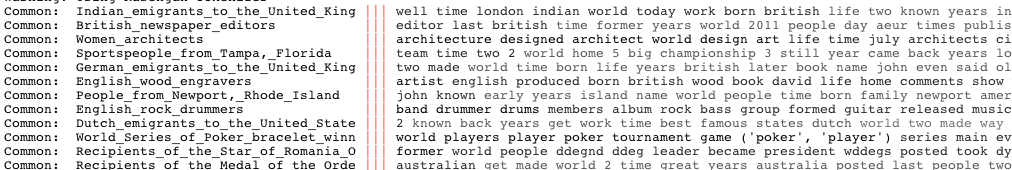
\includegraphics[width=1.18\linewidth]{figures/feature_analysis.png}
  \caption{Naive Bayes Top Features}
  \label{fig:nb-feature-analysis}
\end{adjustwidth}
\end{figure}

We show the performance of this method on the
\textit{catpeople-dev} dataset.
\begin{table}[htbp]
  \centering
\rowcolors{1}{}{lightgrey}
  \begin{tabular}{r  c  c c }\toprule
                  & Feature Selection (Top 20\%) & Feature Selection (Top 70\%) & Feature Selection (Top 60\%) \\
MA-Avg. Prec      & 0.034                        & 0.206                        & 0.197                        \\
MA-Rand-Avg. Prec & 0.013                        & 0.015                        & 0.013                        \\
MA-P-Top10        & 0.203                        & 0.151                        & 0.149                        \\
MA-P-Top10-Rand   & 0.073                        & 0.073                        & 0.073                        \\
MA-P-Top100       & 1.550                        & 0.044                        & 0.046                        \\
MA-P-Top100-Rand  & 0.767                        & 0.843                        & 0.780                        \\
MA-MRR            & 0.094                        & 0.385                        & 0.358                        \\
MA-Rand-MRR       & 0.009                        & 0.009                        & 0.009                        \\
\bottomrule\end{tabular}
  \caption{print 100\% Training. 100 Categories from Dev data.}
  \label{tab:summary-nb}
\end{table}

\begin{table}[htbp]
  \centering
  \begin{tabular}{l | c  | c }\toprule
    Category & MA-AP & MA-AP-Random \\
\verb|Indian_emigrants_to_the_United_Kingdom    |          & 0.013 $\pm$0.002 & 0.039 $\pm$0.010 \\
\verb|British_newspaper_editors                 |          & 0.048 $\pm$0.030 & 0.017 $\pm$0.001 \\
\verb|Women_architects                          |          & 0.188 $\pm$0.110 & 0.013 $\pm$0.005 \\
\verb|Sportspeople_from_Tampa,_Florida          |          & 0.089 $\pm$0.062 & 0.031 $\pm$0.004 \\
\verb|German_emigrants_to_the_United_Kingdom    |          & 0.024 $\pm$0.002 & 0.043 $\pm$0.009 \\
\verb|English_wood_engravers                    |          & 0.081 $\pm$0.056 & 0.024 $\pm$0.011 \\
\verb|People_from_Newport,_Rhode_Island         |          & 0.021 $\pm$0.002 & 0.034 $\pm$0.010 \\
\bullet{\verb|English_rock_drummers             |}         & 0.455 $\pm$0.041 & 0.085 $\pm$0.029 \\
\verb|Dutch_emigrants_to_the_United_States      |          & 0.029 $\pm$0.015 & 0.042 $\pm$0.010 \\
\bullet{\verb|World_Series_of_Poker_bracelet_winners    |} & 0.946 $\pm$0.024 & 0.043 $\pm$0.022 \\
\bottomrule\end{tabular}
  \caption{}
  \label{tab:feat-select-doc-80}
\end{table}
\clearpage
\section{Results with the Multiview
  Alignment Method on Development Data}
\label{sec:results-with-mult}

The Multiview alignment method uses a very different way to determine the
relevance weights for tokens. We first figure out topics for a category. E.g.
for the category \textit{Male\_actors\_from\_Utah} we receive text contexts mentioning
the following actors: Patrick Fugit, Gedde Watanabe, Matthew Davis, Mike
Lookinland, Parley Baer, Art Acord, Richard Harrison, Merlin Olsen, and Joseph
Kearns and we extract the following topics using a generalized set intersection
method:

\begin{table}[htbp]
  \centering
  \begin{tabular}{l c}\toprule
    1. & movie, comedy, cast\\
    2. & film, starring, family\\
    3. & old, time, stars\\
    4. & played, edit\\
    \bottomrule\end{tabular}
  \caption{Topics Found by Generalized Set Interesection Method (Aka Multiview Alignment)}
  \label{tab:topics}
\end{table}
The ranking of these topics is used to weight the individual tokens themselves
in a naive bayes objective where the weight of the tokens belonging to the first
topic is set to 1 and then the weight of tokens belonging to lower ranked topics
decreases.

Using the method described above we obtain the following results on the
development portion of the dataset.


\begin{table}[htbp]
  \centering
  \begin{tabular}{l c}\toprule
    MA-Avg. Prec     & 0.1624\\
MA-Rand-Avg. Prec& 0.0203\\
MA-P-Top10       & 0.1310\\
MA-P-Top10-Rand  & 0.0150\\
MA-P-Top100      & 0.0416\\
MA-P-Top100-Rand & 0.0080\\
MA-MRR           & 0.3531\\
MA-Rand-MRR      & 0.0691\\
    \bottomrule\end{tabular}
  \caption{Retrieval Results on 100 Categories from Dev. Data}
  \label{tab:summary-multiview-alignment}
\end{table}


\clearpage
\bibliographystyle{abbrv}
\bibliography{references}
\end{document}
